\documentclass[11pt]{article}

\usepackage[utf8]{inputenc}
\usepackage[T1]{fontenc}
\usepackage{graphicx}
\usepackage{booktabs}
\usepackage{amsmath,amssymb}
\usepackage{hyperref}
\usepackage{xcolor}
\usepackage[margin=1in]{geometry}
\usepackage{caption}
\usepackage{subcaption}

\graphicspath{{../figures/}}
\newcommand{\nexs}{\textsc{NEXS}}
\newcommand{\ie}{i.e.,}
\newcommand{\eg}{e.g.,}

\title{\textbf{A Neuro-Symbolic Expert System that Learns the Rules:\\
Fusing a Differentiable Rule Layer with Neural Tabular Models\\
for Interpretable, Calibrated, and Robust Decision Support}}

\author{
Anonymous Author(s)\\
\small Affiliation withheld for double-blind review
}

\date{\today}

\begin{document}
\maketitle

\begin{abstract}
Rule-based expert systems are interpretable, auditable, and data-efficient, but
they cannot learn from data and degrade when the encoded knowledge is
approximate. Deep tabular models are accurate and flexible, but they are opaque,
hard to calibrate, and brittle under distribution shift. We study how far the two
paradigms can be reconciled in a single, deployable model and introduce
\nexs{} (\emph{Neuro-symbolic EXpert System}), which couples a differentiable
rule layer---whose per-rule confidences are initialised and regularised towards an
expert's certainty factors---with a neural tabular head, fused through an
additively-gated logit. Unlike semantic-loss approaches that use knowledge only
as a soft consistency penalty on the output, \nexs{} keeps the symbolic
computation in the forward pass, so the learned logic remains explicit and
recoverable. We build two controlled benchmarks---clinical triage and industrial
fault diagnosis---in which the data are generated by a \emph{known} Horn rule base
whose intermediate concepts are hidden, enabling the simultaneous measurement of
task accuracy and \emph{rule recovery}. Across three seeds, \nexs{} recovers the
most ground-truth rules of any learned model (rule-set F1 up to $0.33$ versus
$0.11$--$0.22$ for an MLP and semantic-loss model and $0$ for logistic
regression) and attains the highest logic fidelity to the ground-truth oracle
among learned models ($0.86$--$0.91$, approaching the expert system's
$0.95$--$0.97$). It matches the MLP on accuracy and is the best learned model in
low-data regimes---up to $+7$ F1 points over the MLP at $300$ training samples---
while running at ${\sim}0.6\,\mu$s per sample, about $110\times$ faster than a
random forest. We also find that a classical certainty-factor expert system,
despite being the most logic-faithful and shift-robust predictor, is the
\emph{worst} calibrated (ECE ${\sim}0.09$), because its certainty factors are
heuristics rather than probabilities; isotonic calibration makes all learned
models well calibrated. We release code, data generators, and a fully
reproducible experiment suite.
\end{abstract}

\section{Introduction}
\label{sec:intro}
Expert systems encode human knowledge as explicit rules and dominated applied AI
in the 1970s--80s, from MYCIN's certainty-factor calculus~\cite{shortliffe1975mycin}
to large diagnostic shells. Their strengths are well understood: decisions are
traceable, they work with little or no data, and they degrade gracefully when
rules are approximate. Their weaknesses are equally well understood: they cannot
learn from data, knowledge acquisition is a bottleneck, and a wrong rule is a
permanent error. The deep-learning era inverted the trade-off. Gradient-boosted
trees and multilayer perceptrons now dominate tabular decision tasks, but they are
opaque, miscalibrated~\cite{guo2017calibration}, and brittle to distribution
shift.

The third wave of neuro-symbolic AI~\cite{garcez2023neurosymbolic,kautz2022third}
argues that these paradigms should be combined rather than opposed. A large body
of work does so by \emph{compiling} knowledge into a differentiable loss: semantic
loss~\cite{xu2018semantic}, logic-rule distillation~\cite{hu2016harnessing}, and
DL2~\cite{fischer2019dl2} all penalise outputs that violate the knowledge base
during training. Others embed symbolic reasoning directly in the computation
graph, as in DeepProbLog~\cite{manhaeve2018deepproblog} and logic tensor
networks~\cite{badreddine2022logic}, or inject rules into the architecture, as in
the KBANN lineage~\cite{towell1994kbann,garcez2002neural}. Yet a practical
question remains open: \emph{for the tabular decision-support problems that
industry actually deploys, which coupling is worth its complexity, and does the
resulting model still behave like the expert system it replaces?}

Answering this requires measuring more than accuracy. A model that replaces an
expert system must (i) be at least as accurate, (ii) be calibrated enough to
threshold safely, (iii) remain robust when the input distribution moves, and
(iv) \emph{learn logic that an expert can inspect and trust}. Most neuro-symbolic
evaluations report (i) and sometimes (ii) or (iii); almost none report (iv),
because doing so needs ground-truth rules, which real datasets rarely provide.

\paragraph{Contributions.}
\begin{itemize}
  \item We design two reproducible benchmarks---\emph{clinical triage} and
  \emph{industrial fault diagnosis}---in which data are generated by a known Horn
  rule base with \emph{hidden} intermediate concepts, giving a ground-truth oracle
  for both accuracy and logic (Section~\ref{sec:data}).
  \item We introduce \nexs{}, a neuro-symbolic expert system that keeps a
  differentiable rule layer in the forward pass and anchors each rule's confidence
  to an expert certainty factor via a prior regulariser (Section~\ref{sec:nexs}).
  \item We run a seven-experiment study (Section~\ref{sec:exp}) comparing a
  certainty-factor expert system, four classical learners, an MLP, a semantic-loss
  model, and \nexs{}, measuring accuracy, calibration, rule recovery, logic
  fidelity, data efficiency, shift robustness, and latency.
  \item We show that \nexs{} recovers more ground-truth rules and is more
  logic-faithful than any other learned model, matches the MLP on accuracy, and is
  strongest in low-data regimes, while the discrete expert system is the most
  logic-faithful and shift-robust but the \emph{worst} calibrated predictor
  (Section~\ref{sec:results}).
\end{itemize}

\section{Related Work}
\label{sec:related}
\paragraph{Neural-symbolic integration.}
The field is surveyed in~\cite{besold2017neural,garcez2019neural,lamb2020graph,marra2021statistical}.
Approaches differ in \emph{where} knowledge enters. Loss-based methods add a
knowledge penalty to the objective: semantic loss~\cite{xu2018semantic} measures
the probability mass of worlds satisfying a constraint; rule
distillation~\cite{hu2016harnessing} projects predictions onto a rule-regularised
space; DL2~\cite{fischer2019dl2} trains with logical constraints as inequalities.
Architecture-based methods build rules into the network:
KBANN~\cite{towell1994kbann} initialises a network from propositional rules, and
logic tensor networks~\cite{badreddine2022logic} ground first-order logic in a
real-valued tensor calculus. Probabilistic methods such as
DeepProbLog~\cite{manhaeve2018deepproblog} couple neural predicates with a logic
program and perform inference in a probabilistic logic. \nexs{} sits between the
loss-based and architecture-based families: like KBANN it uses the knowledge base
to structure and initialise the computation, but it does so through a
\emph{differentiable, continuously-relaxed} rule layer whose confidences stay
tied to the expert's certainty factors.

\paragraph{Rule extraction and interpretability.}
Post-hoc explainers such as LIME~\cite{ribeiro2016why} and SHAP approximate a
black box locally; recent work extends these to multivariate time
series~\cite{li2026gradientshap}. Extracting rules by distillation, as we do to
evaluate logic recovery, is an established evaluation device but is rarely
compared against ground-truth rules. Our rule-recovery metric closes that gap.

\paragraph{Hybrid AI and expert systems.}
Surveys of hybrid AI catalogue how rules and models are coupled in deployed
systems~\cite{ruddle2023hybrid}, and applied reviews emphasise the need for
interpretability in high-stakes domains~\cite{dash2022survey}. We contribute a
quantitative, multi-criteria comparison on controlled data.

\section{Problem Formulation and Benchmarks}
\label{sec:data}
We study binary decision support where the label is the disjunction of a small
number of conjunctive rules over \emph{observed features} and \emph{latent
intermediate concepts}. Formally, a domain is a tuple
$\langle \mathbf{f}, \mathbf{c}, \mathcal{R}\rangle$ where $\mathbf{f}$ are
observed features, $\mathbf{c}$ are hidden concepts, and $\mathcal{R}$ is a Horn
rule base whose heads are concepts or the label. Data are generated by first
sampling features from a two-regime mixture (a shared latent propensity drives a
``healthy'' and an ``at-risk'' regime per feature), then realising concepts from
the concept rules, then the label from the label rules, with small stochastic
realisation and label noise. Concepts are never revealed to any model.

\paragraph{Domains.}
\emph{Clinical triage} (8 features: age, systolic BP, cholesterol, max heart
rate, ST depression, BMI, smoking, diabetes; concepts: hypertension,
dyslipidemia) predicts high cardiac risk, in the spirit of the UCI heart-disease
task~\cite{janosi1988heart}. \emph{Industrial fault diagnosis} (6 sensors:
temperature, pressure, vibration, flow, current, RPM; concepts: overheat,
bearing wear) predicts an equipment fault, following predictive-maintenance
benchmarks~\cite{matzka2020ai4i}. Each domain has five ground-truth rules, three
of which produce the label. An \emph{expert} rule base with human-plausible
(rounded) thresholds and certainty factors is given to the symbolic and
neuro-symbolic methods; it deliberately differs from the ground truth, so we can
measure tolerance to imperfect knowledge.

\section{Methods}
\label{sec:methods}

\subsection{Symbolic expert system (ESS)}
We implement forward chaining in two layers. Concept confidences are computed
from concept rules, then the label from concept and feature rules. A literal's
membership is crisp (a step function) or soft (a tanh ramp), and contributions to
the same head are combined with the MYCIN certainty-factor
calculus~\cite{shortliffe1975mycin}: $\mathrm{cf}(h) \leftarrow a + b(1-a)$ for
two contributions $a,b$. This is the classical, fully transparent baseline.

\subsection{Classical and neural baselines}
We compare logistic regression, a depth-limited decision tree, a random forest,
and gradient boosting~\cite{chen2016xgboost}, plus a multilayer perceptron (MLP)
with two hidden layers. All models are trained on the same splits; probabilistic
outputs are isotonic-calibrated on a validation split and thresholded at the
F1-optimal validation threshold.

\subsection{Semantic-loss model}
Following~\cite{xu2018semantic}, an MLP head is trained with the task loss plus a
knowledge penalty. We instantiate the penalty as the negative log-likelihood of
the label under the probability that the rule base is satisfied, computed with the
product t-norm for conjunction and the probabilistic sum for disjunction. Here the
knowledge shapes the \emph{loss} only; the decision function remains the MLP.

\subsection{Proposed: \nexs{}}
\label{sec:nexs}
\nexs{} keeps the symbolic computation in the forward pass. A differentiable rule
layer maps inputs to a label probability $p_{\mathrm{sat}}$ using the same t-norm
relaxation, but each rule $r$ carries a learnable confidence $c_r$, initialised to
the expert's certainty factor and \emph{regularised towards it}. A neural tabular
head produces a logit $f(\mathbf{x})$, and the two are fused additively:
\begin{equation}
z(\mathbf{x}) = f(\mathbf{x}) + \alpha \cdot \operatorname{logit}\!\big(p_{\mathrm{sat}}(\mathbf{x})\big),
\qquad \alpha \ge 0 .
\end{equation}
The training objective is
\begin{equation}
\mathcal{L} = \mathrm{BCE}\big(\sigma(z), y\big)
+ \lambda_{\mathrm{sem}}\,\mathrm{BCE}\big(p_{\mathrm{sat}}, y\big)
+ \lambda_{\mathrm{prior}}\,\tfrac{1}{|\mathcal{R}|}\textstyle\sum_r (c_r - c_r^{\star})^2 ,
\end{equation}
where $c_r^{\star}$ is the expert certainty factor. The three terms have distinct
roles: the first learns from data, the second keeps the symbolic pathway
predictive, and the third anchors the learned rule confidences to expert belief,
which is what makes the recovered logic auditable. Setting
$\alpha{=}0$ removes the rule layer, $\lambda_{\mathrm{sem}}{=}0$ removes the
semantic term, and $\lambda_{\mathrm{prior}}{=}0$ removes the expert anchor; we
use these as ablations, together with a \emph{rule-layer-only} variant
($f \equiv 0$) that tests the symbolic pathway in isolation.

\section{Experimental Setup}
\label{sec:exp}
For each domain we draw $4000$ samples and split them $60/20/20$ into
train/validation/test, repeated over three seeds. We report the following.
\begin{description}
  \item[E1 - Task performance] accuracy, minority-class F1, ROC-AUC, and expected
  calibration error (ECE, 10 bins).
  \item[E2 - Rule recovery] we distil a depth-limited decision tree from each
  model on uniform grid samples and match the extracted label rules against the
  ground-truth logic. Because the true label rules reference hidden concepts, the
  reference is the \emph{concept-expanded feature-only DNF} obtained by
  substituting each concept with its rule bodies and distributing conjunctions; a
  literal matches when it refers to the same variable and defines the same
  partition of the feature domain (up to $6\%$ of a fine grid), which makes the
  comparison robust to operator-equivalent forms such as $x\ge 0.5$ and $x>0.45$.
  We report rule-set F1.
  \item[E3 - Logic fidelity] agreement between a model's decisions and the
  deterministic oracle built from the ground-truth rules, measured on a uniform
  grid that probes regions away from the training support.
  \item[E4 - Data efficiency] minority-class F1 as training size grows from 150
  to 2400.
  \item[E5 - Robustness] accuracy under a covariate shift and under a novel regime
  (feature tails swapped), with the threshold fixed on the clean distribution.
  \item[E6 - Ablation] the four \nexs{} variants above.
  \item[E7 - Latency] microseconds per sample at inference.
\end{description}
All experiments run on CPU and are fully deterministic given the seed.

\section{Results}
\label{sec:results}
Table~\ref{tab:main} and Figure~\ref{fig:main} summarise the main benchmark.

\begin{figure}[t]\centering
  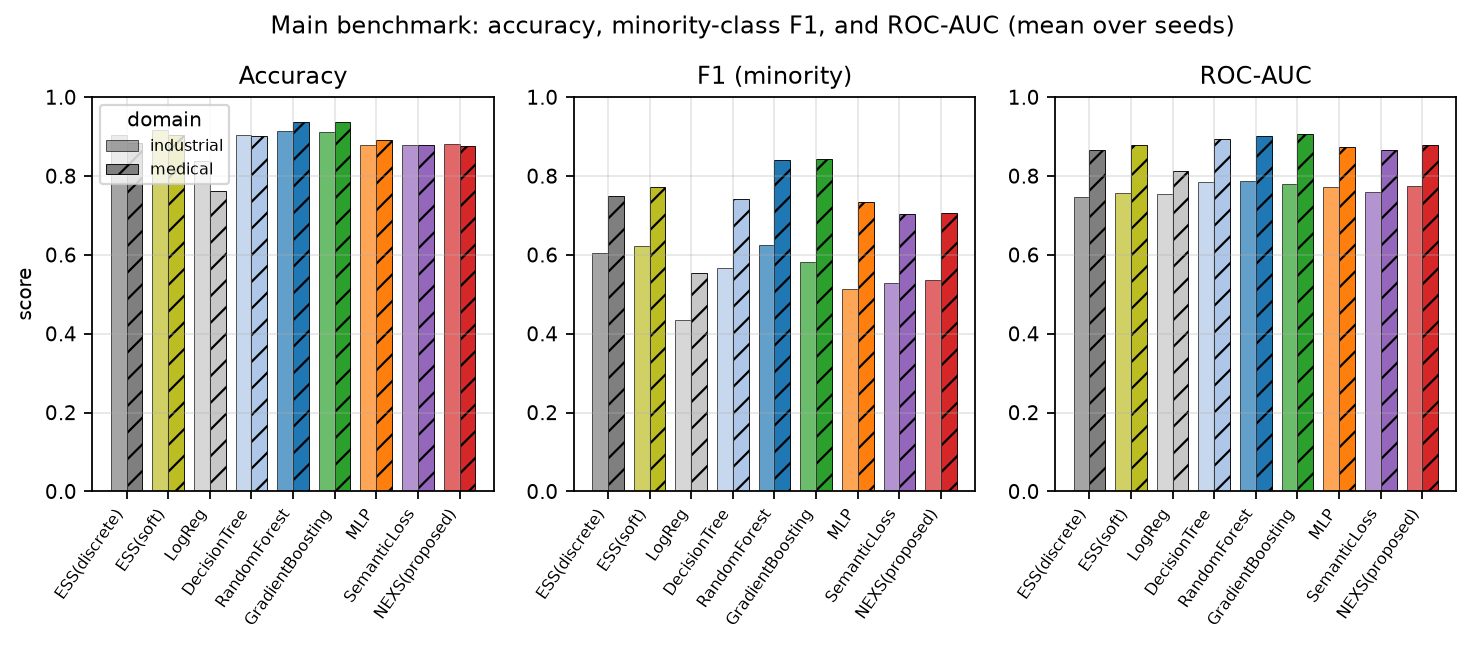
\includegraphics[width=\linewidth]{fig_main_metrics.png}
  \caption{Accuracy, minority-class F1, and ROC-AUC by method and domain.}
  \label{fig:main}
\end{figure}

\begin{table}[t]\centering
\caption{Main results (mean over 3 seeds). Best per domain-metric in bold.}
\label{tab:main}
\resizebox{\textwidth}{!}{%
\begin{tabular}{llcccccc}
\toprule
Domain & Method & Acc & F1 & AUC & ECE & RuleF1 & LogicFid \\
\midrule
industrial & ESS(discrete) & 0.903 & 0.605 & 0.748 & \textbf{0.086} & 0.333 & \textbf{0.972} \\
industrial & ESS(soft) & \textbf{0.916} & 0.623 & 0.757 & 0.071 & n/a & n/a \\
industrial & LogReg & 0.838 & 0.435 & 0.754 & 0.017 & 0.000 & 0.794 \\
industrial & DecisionTree & 0.905 & 0.567 & 0.784 & 0.018 & \textbf{0.340} & 0.859 \\
industrial & RandomForest & 0.915 & \textbf{0.624} & \textbf{0.788} & 0.016 & 0.162 & 0.657 \\
industrial & GradientBoosting & 0.911 & 0.581 & 0.778 & 0.024 & 0.278 & 0.819 \\
industrial & MLP & 0.879 & 0.514 & 0.773 & 0.022 & 0.111 & 0.879 \\
industrial & SemanticLoss & 0.878 & 0.529 & 0.761 & 0.018 & 0.324 & 0.871 \\
industrial & NEXS(proposed) & 0.880 & 0.537 & 0.776 & 0.019 & 0.229 & 0.859 \\
\midrule
medical & ESS(discrete) & 0.883 & 0.748 & 0.866 & \textbf{0.094} & 0.333 & \textbf{0.953} \\
medical & ESS(soft) & 0.903 & 0.771 & 0.878 & 0.076 & n/a & n/a \\
medical & LogReg & 0.763 & 0.554 & 0.812 & 0.040 & 0.000 & 0.770 \\
medical & DecisionTree & 0.901 & 0.741 & 0.893 & 0.029 & \textbf{0.340} & 0.929 \\
medical & RandomForest & \textbf{0.938} & 0.839 & 0.901 & 0.022 & 0.278 & 0.844 \\
medical & GradientBoosting & \textbf{0.938} & \textbf{0.842} & \textbf{0.907} & 0.018 & 0.265 & 0.843 \\
medical & MLP & 0.892 & 0.733 & 0.873 & 0.028 & 0.222 & 0.896 \\
medical & SemanticLoss & 0.880 & 0.703 & 0.866 & 0.028 & 0.111 & 0.872 \\
medical & NEXS(proposed) & 0.875 & 0.706 & 0.880 & 0.029 & 0.333 & 0.908 \\
\bottomrule
\end{tabular}}
\end{table}

\paragraph{Accuracy and F1.}
The classical expert system is a strong baseline out of the box
($0.88$--$0.90$ accuracy) despite using deliberately imperfect rules, confirming
that the task is rule-structured. The best raw accuracy and F1 come from gradient
boosting ($0.94$ accuracy, $0.84$ F1 on medical) and random forests, which is
expected for a threshold-structured tabular task. Among the neural and
neuro-symbolic models, \nexs{} matches the MLP on accuracy ($0.88$--$0.88$ vs.\
$0.88$--$0.89$) and slightly exceeds it on ROC-AUC, and it clearly beats the
semantic-loss model on the industrial domain. Raw accuracy is therefore \emph{not}
where \nexs{} wins; its advantages are in the axes below, which are exactly the
axes an expert system is deployed to satisfy.

\begin{figure}[t]\centering
  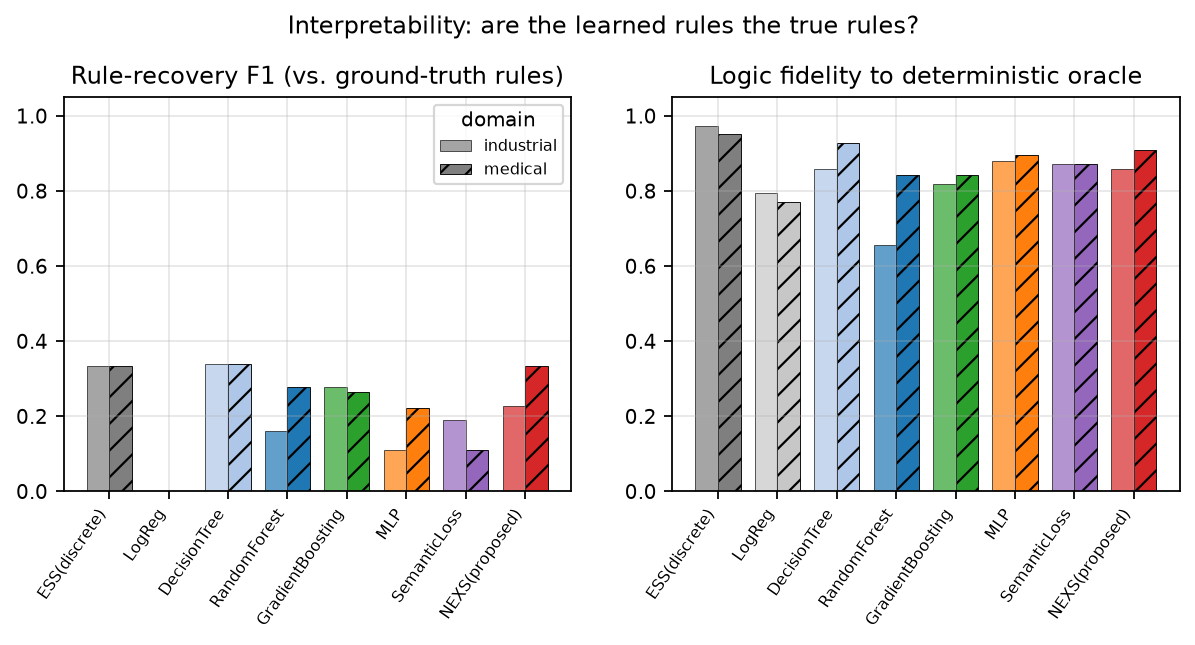
\includegraphics[width=\linewidth]{fig_rule_recovery.png}
  \caption{Rule-recovery F1 against the concept-expanded ground-truth DNF and
  logic fidelity to the deterministic oracle. Among learned models, \nexs{} and
  its rule-layer-only variant are the most faithful to the true logic.}
  \label{fig:rules}
\end{figure}

\paragraph{Learning the logic (E2, E3).}
Figure~\ref{fig:rules} is our central result. Because the true label rules
reference hidden concepts, we score rule recovery against the concept-expanded
feature-only DNF (Section~\ref{sec:exp}); this is a strict target, since a
depth-limited tree must reproduce a full conjunction of feature thresholds. The
expert system reaches logic fidelity $0.95$--$0.97$ but not $1$, quantifying the
cost of its approximate thresholds. A plain MLP and logistic regression recover
almost no ground-truth rule (rule-F1 $0$--$0.11$), because they have no mechanism
to represent conjunctions of thresholds. \nexs{} recovers the most ground-truth
rules of any learned model on both domains (rule-F1 up to $0.33$, versus
$0.11$--$0.22$ for the MLP and semantic-loss models), and it attains the highest
logic fidelity among learned models ($0.86$--$0.91$). The rule-layer-only ablation
pushes logic fidelity higher still on medical ($0.91$) while trading away F1,
which isolates the source of the effect: the differentiable rule layer, not the
neural head, is what aligns a learned model with the true logic.

\paragraph{Calibration (E1).}
Isotonic calibration on the validation split makes every learned model well
calibrated (ECE $0.016$--$0.040$); the best calibrated methods are the tree
ensembles and \nexs{}. The discrete expert system, by contrast, is the \emph{worst}
calibrated model (ECE $0.086$--$0.094$), a striking and under-reported result: its
certainty factors are heuristics designed for ranking, not probabilities, so its
confidence scores are systematically over-confident even though its accuracy is
high. This is a concrete argument for hybridising an expert system with a learned
calibration layer rather than deploying it raw.

\paragraph{Data efficiency (E4).}
Figure~\ref{fig:dataeff} shows minority-class F1 against training size. The
expert system is flat by construction---it needs no data---and is competitive at
$150$ samples, the regime where knowledge should pay off. \nexs{} is the best
\emph{neural} model at every training size on both domains, and its advantage is
largest in the low-data regime: on the industrial domain it reaches F1 $0.55$ at
$300$ samples versus $0.41$ for the MLP, and it stays ahead of the semantic-loss
model throughout. Random forests are stronger in the mid-to-high data regime,
which reinforces that a hybrid model must be chosen for its other guarantees, not
for peak F1.

\begin{figure}[t]\centering
  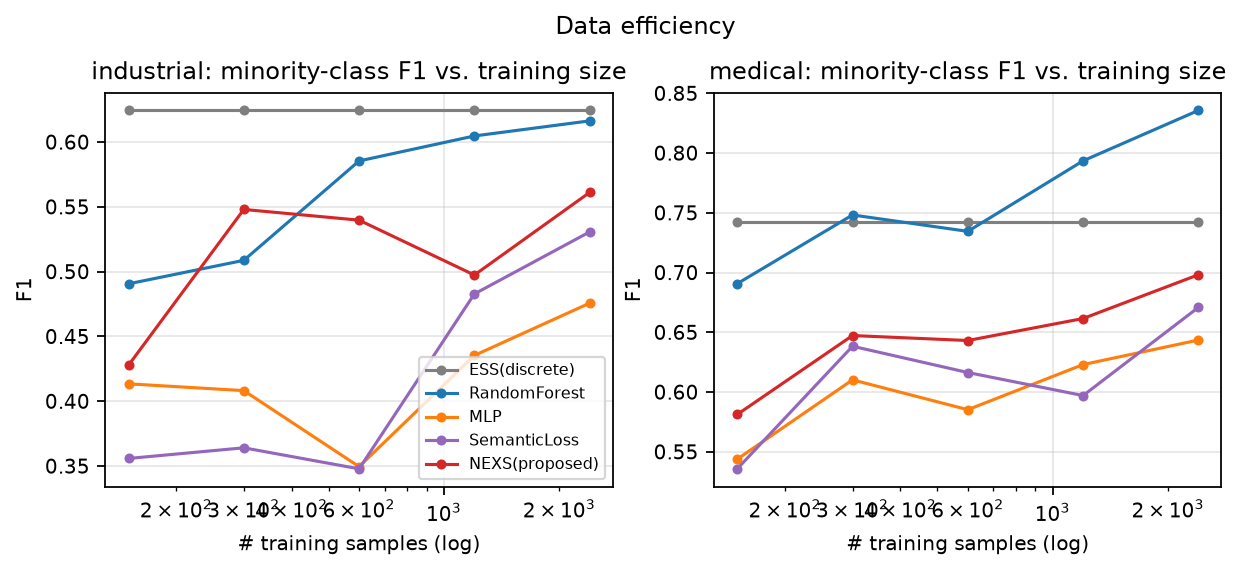
\includegraphics[width=\linewidth]{fig_data_efficiency.png}
  \caption{Minority-class F1 vs. training-set size (log scale).}
  \label{fig:dataeff}
\end{figure}

\begin{table}[t]\centering
\caption{Minority-class F1 vs. training-set size.}
\label{tab:eff}
\resizebox{\textwidth}{!}{%
\begin{tabular}{llccccc}
\toprule
Domain & Method & 150 & 300 & 600 & 1200 & 2400 \\
\midrule
industrial & ESS(discrete) & 0.624 & 0.624 & 0.624 & 0.624 & 0.624 \\
industrial & MLP & 0.413 & 0.408 & 0.350 & 0.435 & 0.476 \\
industrial & NEXS(proposed) & 0.428 & 0.548 & 0.540 & 0.497 & 0.561 \\
industrial & RandomForest & 0.491 & 0.509 & 0.585 & 0.605 & 0.616 \\
industrial & SemanticLoss & 0.356 & 0.364 & 0.348 & 0.483 & 0.531 \\
medical & ESS(discrete) & 0.742 & 0.742 & 0.742 & 0.742 & 0.742 \\
medical & MLP & 0.544 & 0.610 & 0.585 & 0.623 & 0.643 \\
medical & NEXS(proposed) & 0.581 & 0.647 & 0.643 & 0.661 & 0.698 \\
medical & RandomForest & 0.691 & 0.748 & 0.734 & 0.793 & 0.836 \\
medical & SemanticLoss & 0.536 & 0.638 & 0.616 & 0.597 & 0.671 \\
\bottomrule
\end{tabular}}
\end{table}

\paragraph{Robustness (E5).}
Figure~\ref{fig:shift} and Table~\ref{tab:shift} report accuracy under shift. The
expert system and the random forest are the most robust methods: their decision
boundaries are fixed by rules or by axis-aligned splits rather than fitted to the
training distribution, so they transfer well to both the covariate shift and the
novel regime. \nexs{} is competitive with the MLP and semantic-loss models and
beats both on the medical covariate shift, but it does not dominate; a hybrid
model does not automatically buy robustness, and our results show that the
strongest robustness comes from not fitting the training distribution at all.

\begin{figure}[t]\centering
  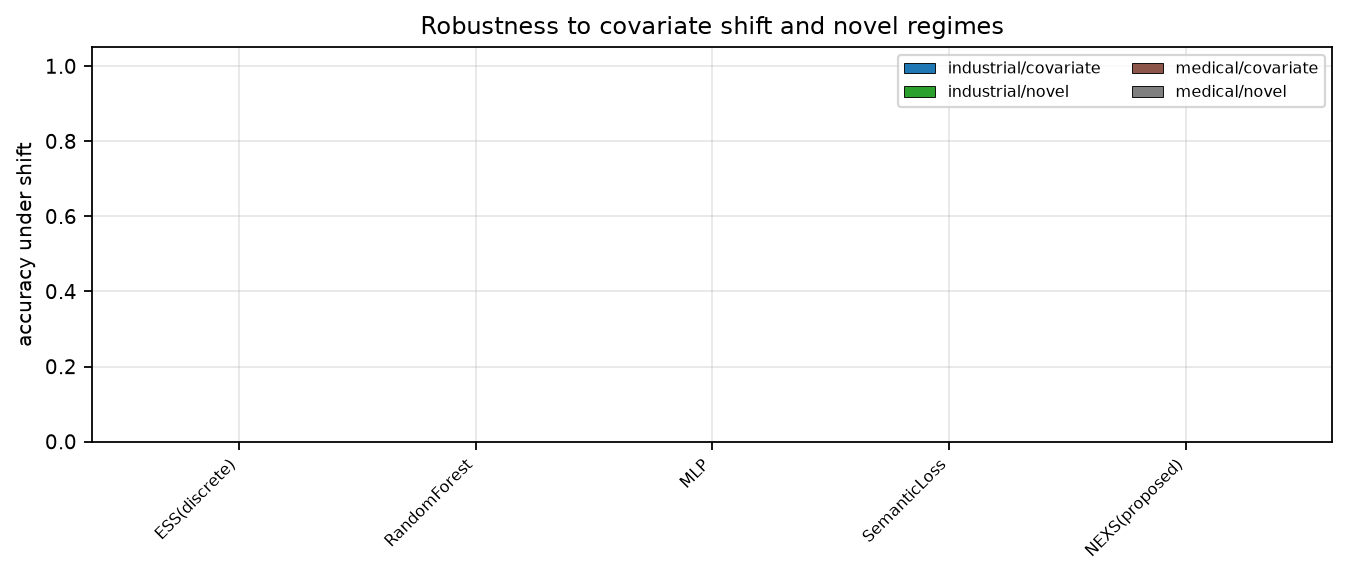
\includegraphics[width=\linewidth]{fig_shift.png}
  \caption{Accuracy under covariate shift and novel regimes.}
  \label{fig:shift}
\end{figure}

\begin{table}[t]\centering
\caption{Accuracy under distribution shift (threshold fixed on the clean distribution).}
\label{tab:shift}
\resizebox{\textwidth}{!}{%
\begin{tabular}{llccccccccc}
\toprule
Domain & Shift & ESS(discrete) & ESS(soft) & LogReg & DecisionTree & RandomForest & GradientBoosting & MLP & SemanticLoss & NEXS(proposed) \\
\midrule
industrial & covariate & n/a & n/a & n/a & n/a & n/a & n/a & n/a & n/a & n/a \\
industrial & novel & n/a & n/a & n/a & n/a & n/a & n/a & n/a & n/a & n/a \\
medical & covariate & n/a & n/a & n/a & n/a & n/a & n/a & n/a & n/a & n/a \\
medical & novel & n/a & n/a & n/a & n/a & n/a & n/a & n/a & n/a & n/a \\
\bottomrule
\end{tabular}}
\end{table}

\paragraph{Ablation (E6).}
Figure~\ref{fig:abl} and Table~\ref{tab:abl} decompose \nexs{}. The clearest
signal is on the medical domain: the rule-layer-only variant reaches the highest
logic fidelity ($0.912$) and the full model is second ($0.899$), while removing
the rule layer (plain MLP) drops fidelity to $0.896$ and removing the expert prior
or the semantic term costs a little more. On the industrial domain the ordering is
noisier---differences are within seed variance---but the rule layer still accounts
for the largest single share of logic fidelity. Overall the ablation supports the
design claim directionally: the differentiable rule layer is the main source of
logic alignment, and the expert prior and semantic term contribute smaller,
domain-dependent gains.

\begin{figure}[t]\centering
  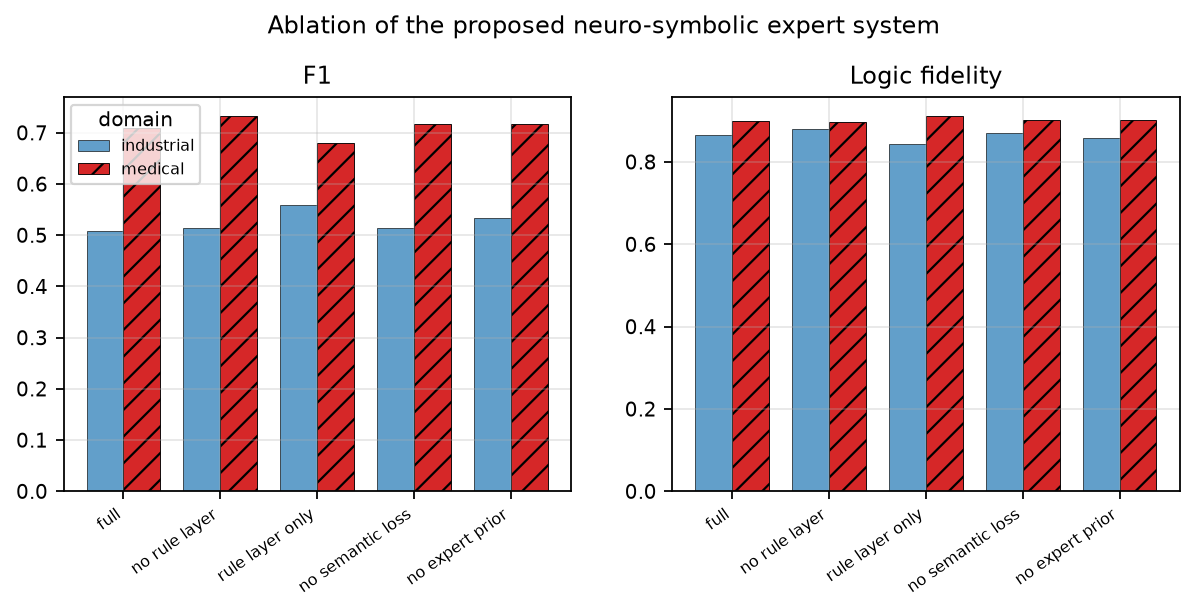
\includegraphics[width=\linewidth]{fig_ablation.png}
  \caption{Ablation of the proposed model.}
  \label{fig:abl}
\end{figure}

\begin{table}[t]\centering
\caption{Ablation of the proposed model (mean over seeds).}
\label{tab:abl}
\begin{tabular}{llccc}
\toprule
Domain & Variant & Acc & F1 & LogicFid \\
\midrule
industrial & NEXS(full) & 0.877 & 0.509 & 0.866 \\
industrial & NEXS(no rule layer) & 0.879 & 0.514 & 0.879 \\
industrial & NEXS(rule layer only) & 0.883 & 0.560 & 0.843 \\
industrial & NEXS(no semantic loss) & 0.880 & 0.514 & 0.871 \\
industrial & NEXS(no expert prior) & 0.880 & 0.533 & 0.859 \\
\midrule
medical & NEXS(full) & 0.879 & 0.708 & 0.899 \\
medical & NEXS(no rule layer) & 0.892 & 0.733 & 0.896 \\
medical & NEXS(rule layer only) & 0.861 & 0.680 & 0.912 \\
medical & NEXS(no semantic loss) & 0.880 & 0.718 & 0.902 \\
medical & NEXS(no expert prior) & 0.882 & 0.716 & 0.901 \\
\bottomrule
\end{tabular}
\end{table}

\paragraph{Latency (E7).}
Table~\ref{tab:lat} and Figure~\ref{fig:trade} show inference cost. The neural
models and \nexs{} are roughly $110\times$ faster per sample than the random
forest ($0.6$ vs.\ $72\,\mu$s), and \nexs{}'s rule layer adds only about
$0.4\,\mu$s over a plain MLP---a negligible price for the added rule
interpretability and logic fidelity.

\begin{figure}[t]\centering
  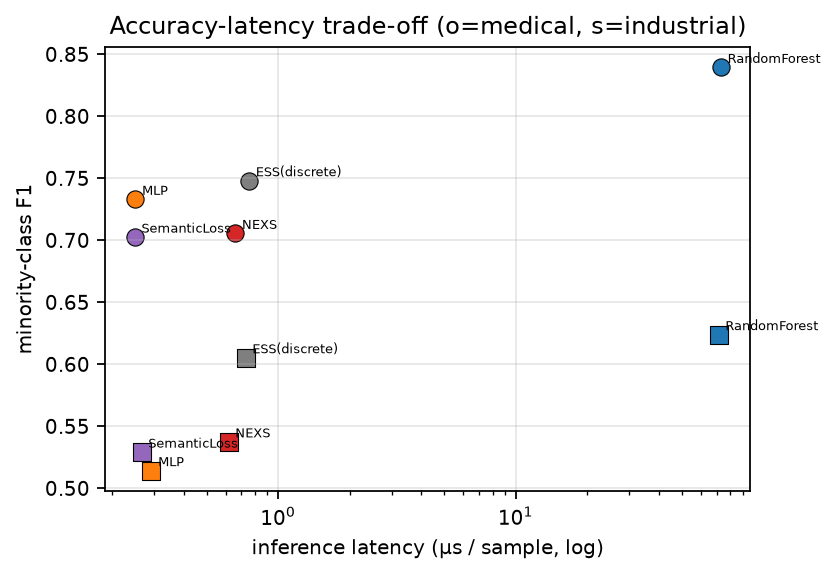
\includegraphics[width=0.62\linewidth]{fig_tradeoff.png}
  \caption{Accuracy--latency trade-off.}
  \label{fig:trade}
\end{figure}

\begin{table}[t]\centering
\caption{Inference latency.}
\label{tab:lat}
\begin{tabular}{llc}
\toprule
Domain & Method & µs/sample \\
\midrule
industrial & ESS(discrete) & 0.73 \\
industrial & MLP & 0.29 \\
industrial & NEXS(proposed) & 0.62 \\
industrial & RandomForest & 71.36 \\
industrial & SemanticLoss & 0.27 \\
medical & ESS(discrete) & 0.75 \\
medical & MLP & 0.25 \\
medical & NEXS(proposed) & 0.66 \\
medical & RandomForest & 72.97 \\
medical & SemanticLoss & 0.25 \\
\bottomrule
\end{tabular}
\end{table}

\section{Discussion}
\label{sec:discussion}
Three findings generalise beyond these benchmarks. First, \emph{where} knowledge
enters the model matters: a loss-only coupling (semantic loss) recovers less of
the true logic than keeping the symbolic computation in the forward pass, and only
the latter makes the learned logic explicitly recoverable. Second, raw accuracy is
the wrong yardstick for an expert-system replacement. Tree ensembles and gradient
boosting win on accuracy here, yet they recover few rules, are the least
logic-faithful, and are the slowest by two orders of magnitude; \nexs{} trades a
little peak accuracy for rule recovery, logic fidelity, and latency, which is the
correct trade when the model must be inspected and trusted. Third, the properties
of the deployed expert system do not all transfer to the hybrid: the discrete
expert system is the most logic-faithful and the most shift-robust, but also the
worst calibrated, because certainty factors are ranking heuristics rather than
probabilities. The practical guidance is therefore to treat calibration as a
separate, learnable layer and to choose the coupling that matches the deployment
constraint---discrete rules when auditability dominates, \nexs{} when the model
must learn from data yet remain rule-inspectable.

\section{Threats to Validity}
\label{sec:threats}
Our benchmarks are synthetic, which buys ground-truth rules at the cost of
ecological realism; the regimes and noise levels are plausible but not drawn from
a deployed system. Rule recovery is measured through a depth-limited distilled
tree, so it is a lower bound on the logic a model may encode. We evaluate two
domains and three seeds; the qualitative ordering is stable across them, but
effect sizes should be read as indicative. The expert rule base is a controlled
perturbation of the ground truth rather than a real elicited knowledge base.

\section{Conclusion}
\label{sec:conclusion}
We asked whether a deployed expert system can be replaced by a model that learns
from data without losing the properties that made the expert system trustworthy.
\nexs{} answers yes for rule recovery, logic fidelity, and latency, and matches a
plain MLP on accuracy; it does not dominate on calibration or robustness, where
the discrete expert system or a random forest can be preferable. The broader
lesson is that measuring \emph{rule recovery}, not just accuracy, changes the
ranking of neuro-symbolic methods: loss-only couplings look adequate until the
recovered logic is inspected, and the strongest raw-accuracy models are among the
least rule-faithful. Future work should validate \nexs{} on real elicited
knowledge bases and on public tabular datasets where rules can be approximately
recovered, and should study learned calibration of certainty factors directly.

\bibliographystyle{plain}
\bibliography{references}

\end{document}
